
\newpage

\ESKDthisStyle{formII}
\ESKDcolumnII{ПРИЛОЖЕНИЕ A}
\begingroup
  % тут добавляем \centering в before-code
  \titleformat{\section}[block]
    {\normalfont\bfseries} % формат (оставляем обычный)
    {\thesection}          % номер секции
    {0.5em}                % отступ между номером и текстом
    {\centering}           % before-code: теперь центрируем
  \section*{ПРИЛОЖЕНИЕ A}
\endgroup
\addcontentsline{toc}{section}{ПРИЛОЖЕНИЕ A}

\setcounter{figure}{0} 
\makeatletter
  \renewcommand{\thefigure}{A.\arabic{figure}}
\makeatother


\begin{figure}[h]
\centering
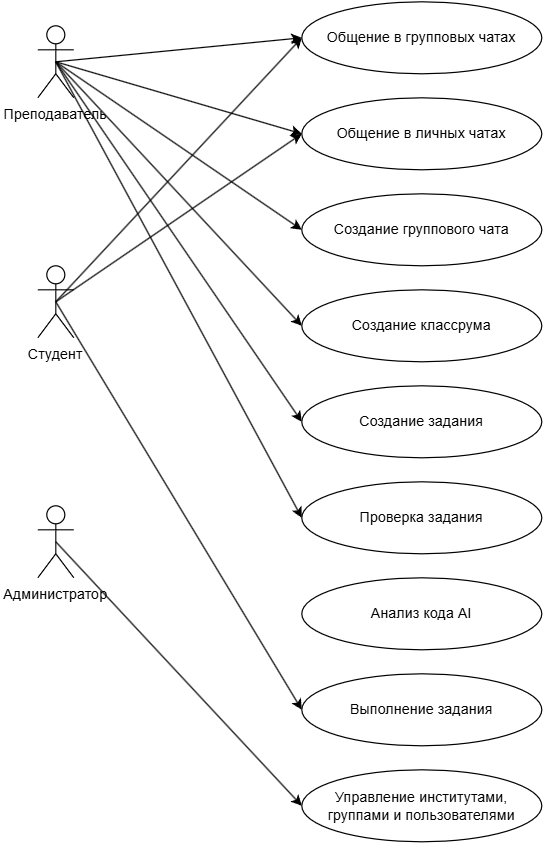
\includegraphics[width=0.5\linewidth]{static/useCaseDiagramm}
\caption{Диаграмма вариантов использования системы для различных ролей пользователей.}
\label{fig:usecasediagramm}
\end{figure}

\begin{figure}[h]
    \centering
    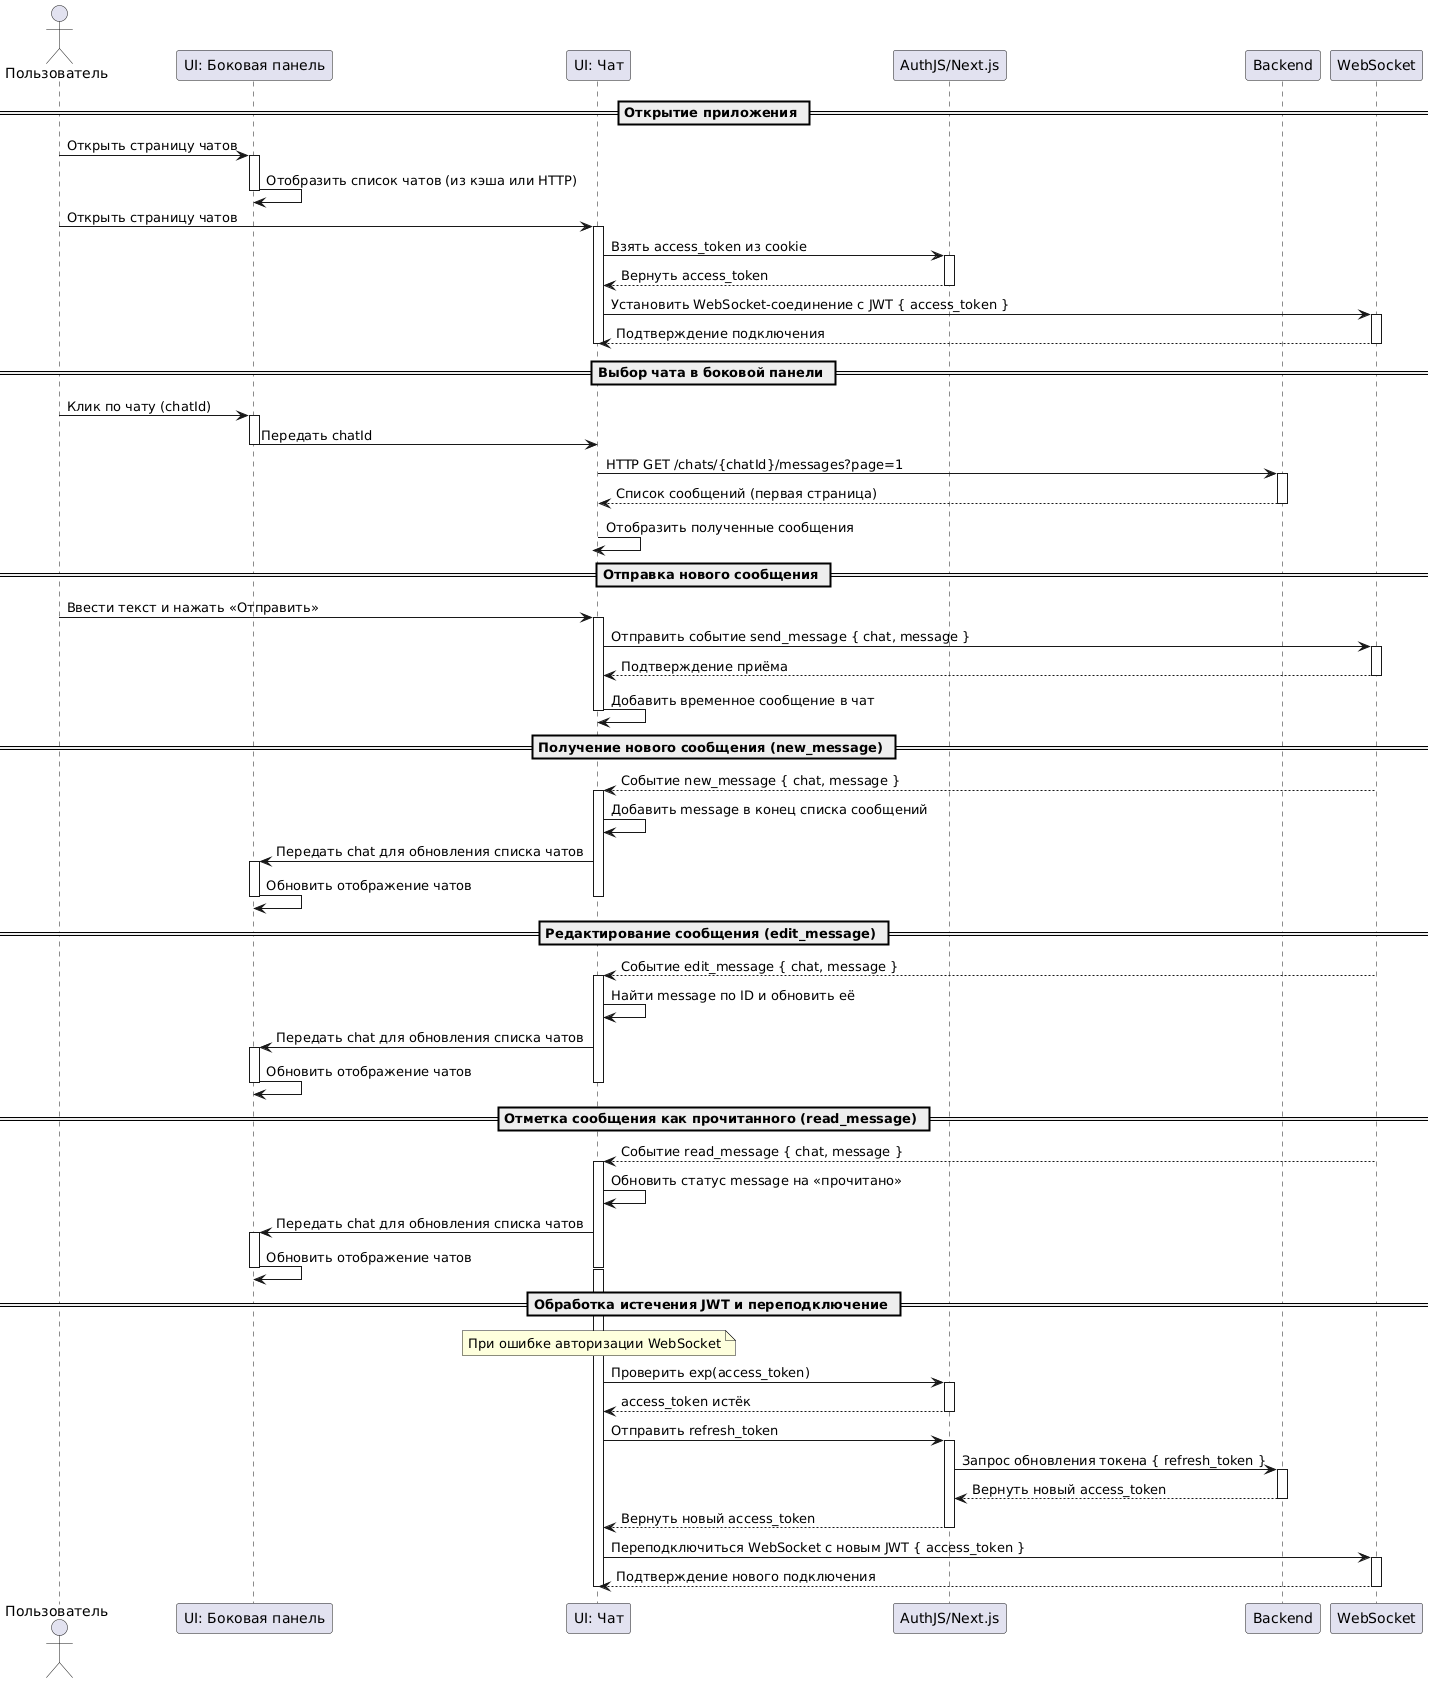
\includegraphics[width=0.9\textwidth]{static/diagrams/Chats.png}
    \caption{Схема взаимодействия клиента (UI: Боковая панель и UI: Чат), AuthJS (Next.js), бэкенда и WebSocket при работе модуля «Chats».}
    \label{fig:chats-flow}
\end{figure}


\begin{figure}[h]
    \centering
    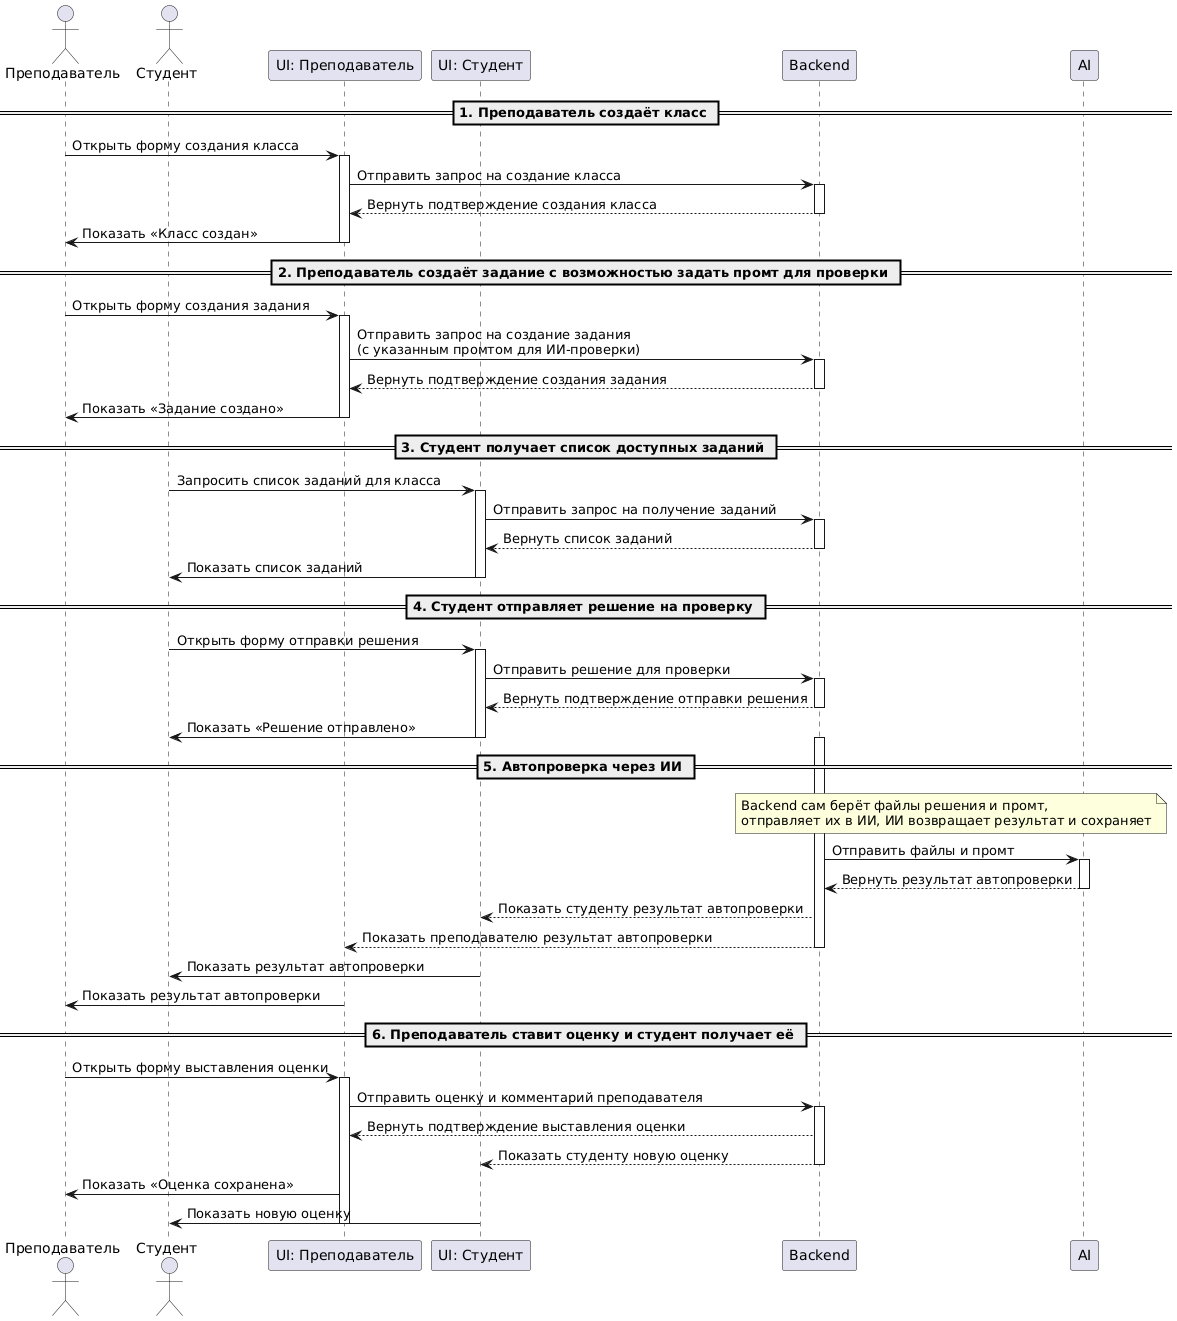
\includegraphics[width=0.9\textwidth]{static/diagrams/Classroom.png}
    \caption{Схема взаимодействия преподавателя, студента, и искуственного интелекта при работе с виртуальными классами}
    \label{fig:classroom-flow}
\end{figure}

  
\begin{figure}[h]
	\centering
	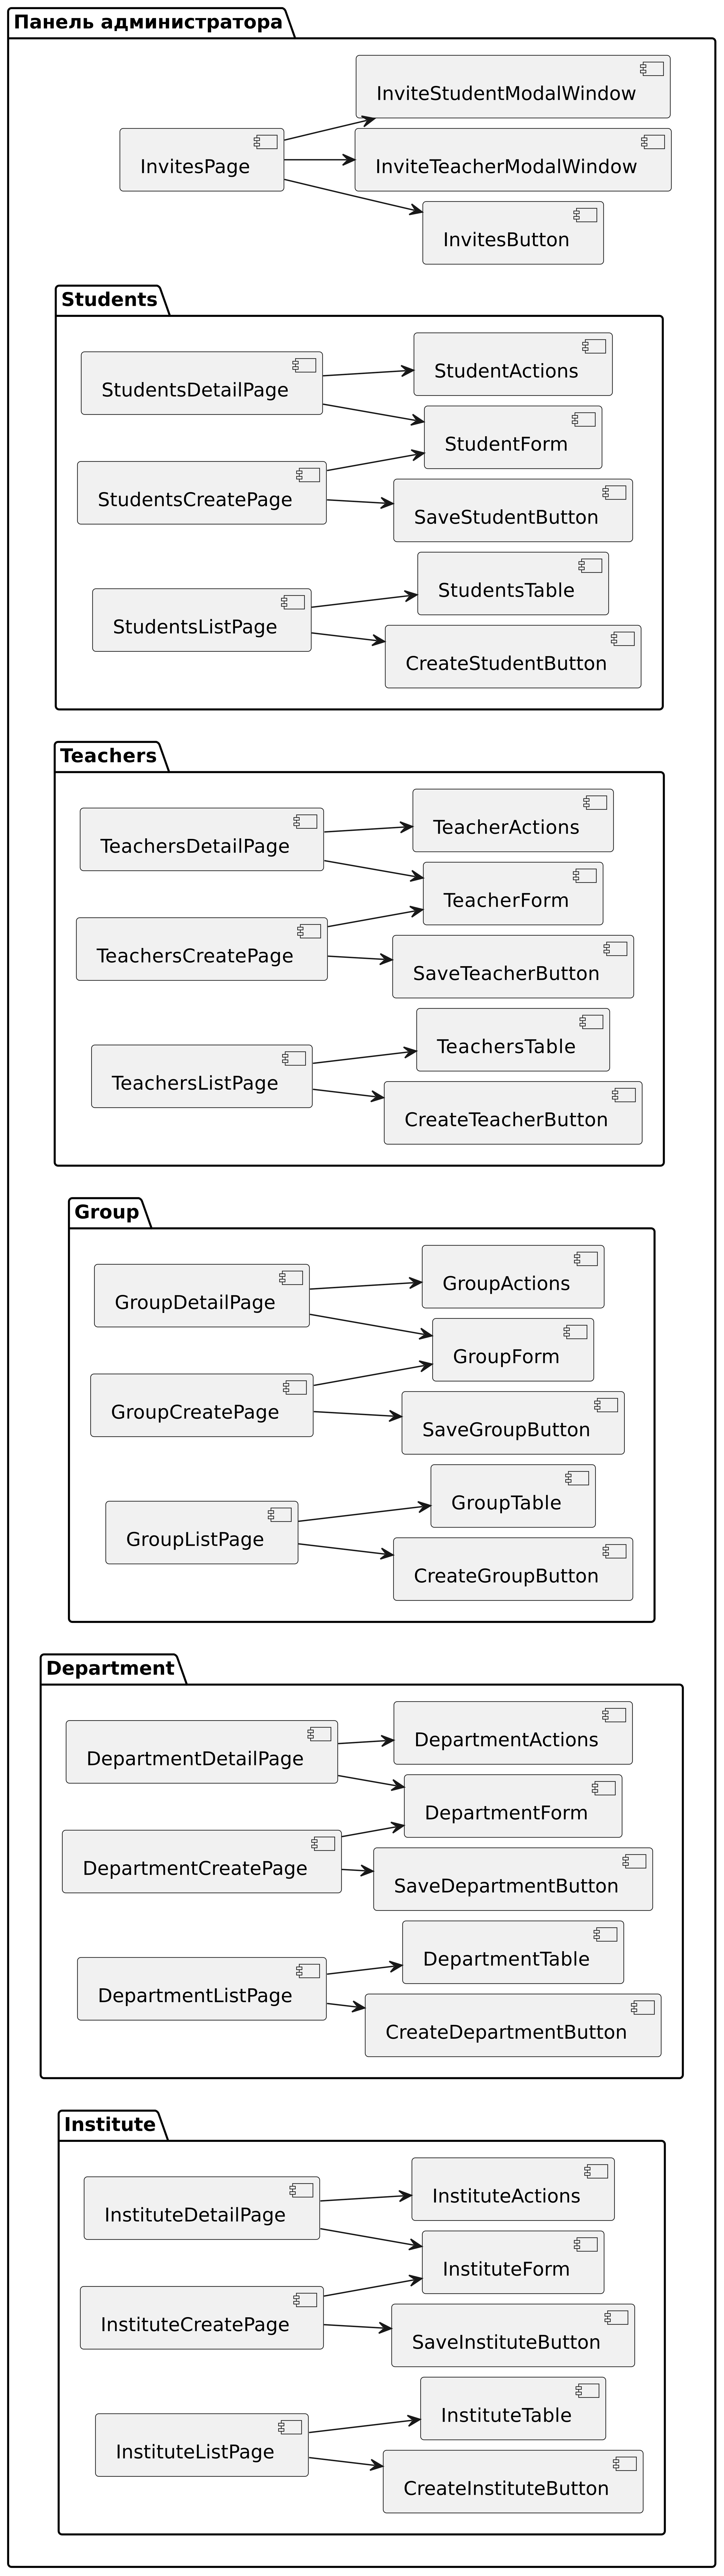
\includegraphics[width=0.4\textwidth]{static/diagrams/AdminComponentDiagram.png}
	\caption{Диаграмма компонентов административной панели}
	\label{fig:admin-components}
\end{figure}

\begin{figure}[h]
  \centering
  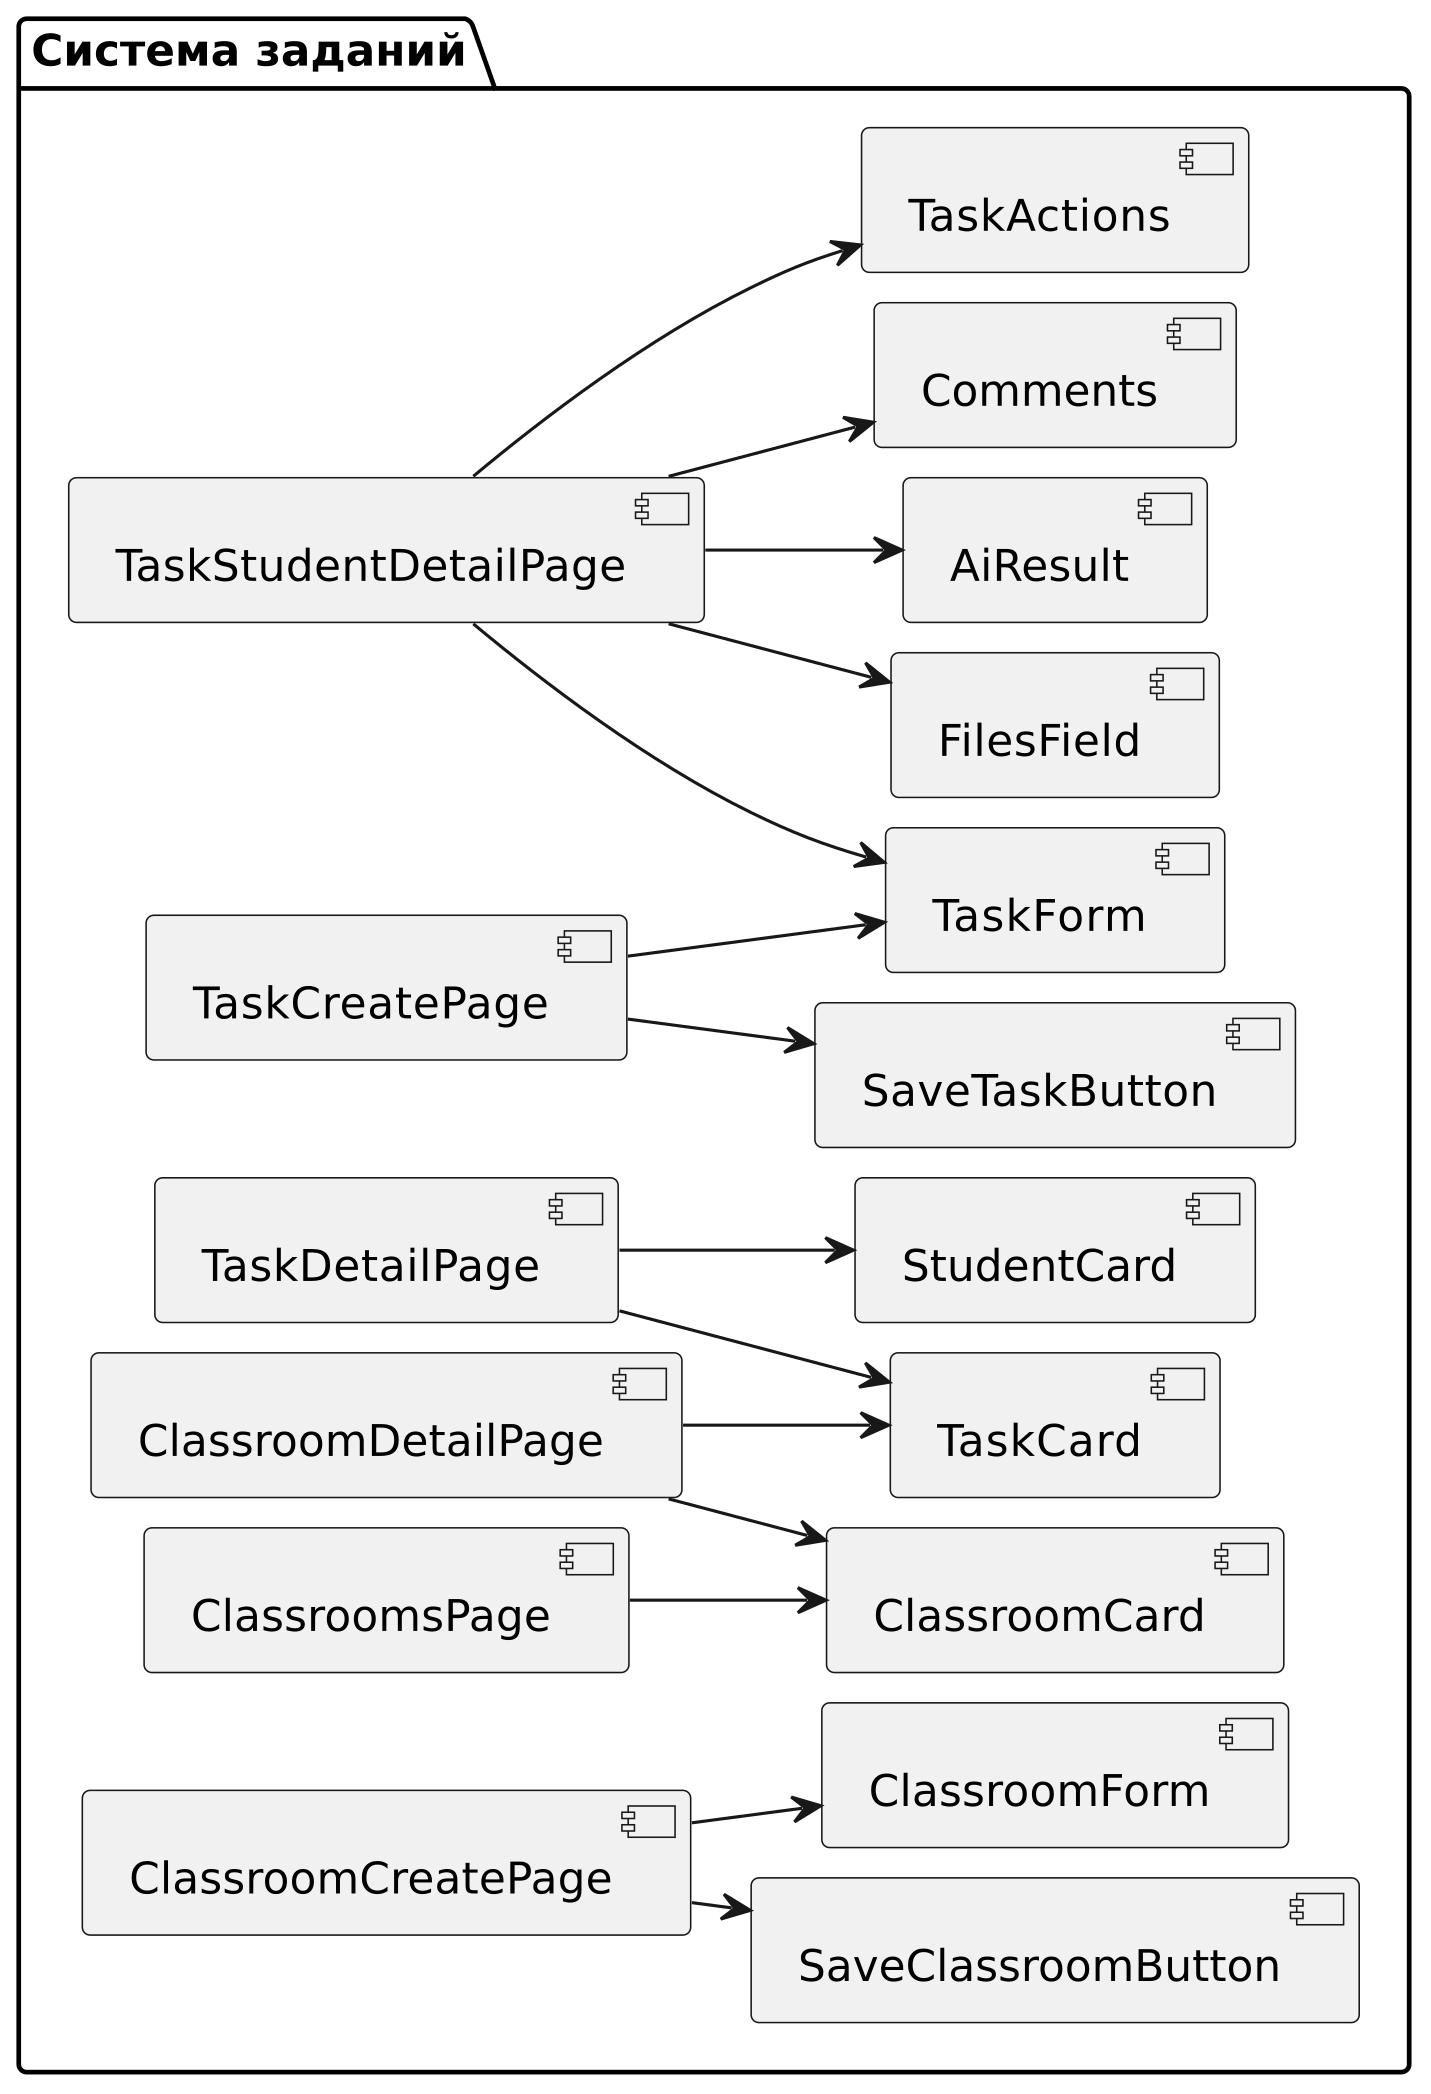
\includegraphics[width=0.7\textwidth]{static/diagrams/ClassroomComponentDiagram.png}
  \caption{Диаграмма компонентов системы заданий}
  \label{fig:classroom-components}
\end{figure}
  
\ESKDthisStyle{formII}
\ESKDcolumnII{ПРИЛОЖЕНИЕ Б}
\begingroup
  % тут добавляем \centering в before-code
  \titleformat{\section}[block]
    {\normalfont\bfseries} % формат (оставляем обычный)
    {\thesection}          % номер секции
    {0.5em}                % отступ между номером и текстом
    {\centering}           % before-code: теперь центрируем
  \section*{ПРИЛОЖЕНИЕ Б}
\endgroup
\addcontentsline{toc}{section}{ПРИЛОЖЕНИЕ Б}
\begin{center}
\textbf{Исходный код программы}
\end{center}
По результатам данной работы был реализовано front-end часть приложения. Ознакомится с исходным кодом приложения можно по \href{https://github.com/BeSmileV/unichat-front}{ссылке на репозиторий GitHub}.

